\documentclass[11pt,a4paper]{article}
\usepackage{solutions}
\newcommand{\q}[1]{\par\medskip\noindent\textbf{#1.}\enspace}
\newcommand{\vv}[1]{\vec{#1}}
\begin{document}
\doctitle{Physics A}{PC track \,$\cdot$\, Paper no.~3 \,$\cdot$\, Tuesday 14 April 2026, 08:00--12:00}
         {Duration: 4 hours. The use of calculators is not allowed for this paper.}
         {English translation}

\begin{remark}
Unofficial English translation of the original French paper
(\texttt{physique-a-pc\_paper\_fr.pdf}, in this folder). Question numbers, notation and figures
are unchanged. In case of doubt, the French original prevails.
\end{remark}

\begin{center}
{\large\bfseries Modern techniques for the mass spectrometry of complex molecules}\\[6pt]
\emph{The two parts are independent.}\\
\emph{Most of the questions can be answered concisely.}
\end{center}

Identifying complex molecules is an important challenge in chemistry and biology. It often
relies on a precise measurement of the mass of the molecule, from which its molecular formula
can be deduced. The measurement is carried out in two steps. First, one or more electrons are
removed from the molecule. Second, the trajectory of the ion thus formed in an electromagnetic
field is studied by means of a mass spectrometer.

Various techniques are used for each of these two steps. In the first part, we study
electrospray ionisation, known by its acronym ESI, which earned its inventor, the American
John Fenn, the Nobel Prize in Chemistry in 2002. This technique ionises very large molecules
without breaking them, and naturally produces highly charged ions, which guarantee a more
precise measurement. In the second part, we study so-called ``ion cyclotron resonance'' mass
spectrometry, known by its acronym FT-ICR-MS, which is very precise and can analyse a large
number of compounds present in a sample simultaneously.

\begin{center}\bfseries I -- Electrospray ionisation\end{center}

Electrospray is an electrostatic method. A high potential difference (a few kV) is applied
between the end of a small steel tube, called a capillary tube, and an electrode located near
the outlet of the tube. A conducting liquid containing the substance under study flows very
slowly through the tube. The electric field pulls on the surface of the liquid leaving the
tube, which then forms an almost perfect, stationary cone (figure~1). A thin jet leaves the
tip of this liquid cone and then breaks up into microscopic charged droplets. The evaporation
of these droplets leads to isolated ions, which are sent into the spectrometer.

\begin{center}
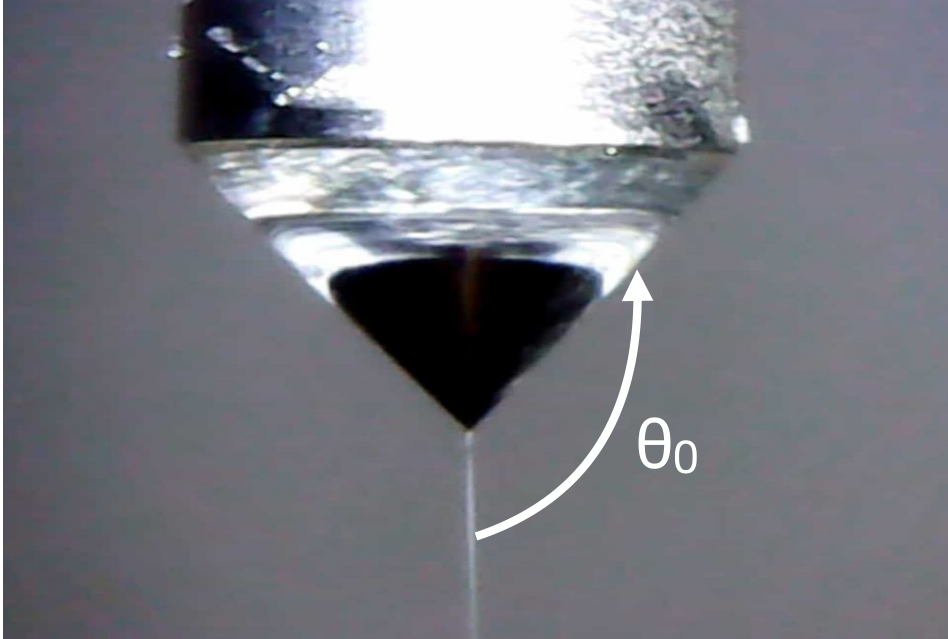
\includegraphics[width=0.46\textwidth]{fig/fig1-taylor-cone.png}
\end{center}
\noindent\small\textsc{Figure 1} -- An electrospray source showing, from top to bottom: the
capillary tube inside which the liquid under study flows (diameter 0.2~mm); the cone formed by
the liquid leaving the tube under the effect of the electrostatic force; and the thin jet coming
from the tip of the cone. The break-up of this jet produces the ions that will be sent into the
mass spectrometer. [Illustration adapted from
\texttt{https://sprucescience.com/products/taylor-cone/}]\normalsize

\subpart{Parallel-plate capacitor}
We first derive the expression of the electrostatic force exerted on a plate of a
parallel-plate capacitor.

\q{1} Recall the relation between the surface charge density on one of the plates, denoted
$\sigma$, and the electric field $E$ between the plates.

\q{2} Recall the expression of the electrostatic energy per unit volume in terms of $E$.

\q{3} Deduce the force per unit area, denoted $P$, exerted on one of the plates of the
capacitor, and give its direction. Express $P$ in terms of $E$, then in terms of $\sigma$.

We shall accept that the expressions of $P$ thus obtained remain valid at every point of the
surface of a conductor of arbitrary shape in electrostatics: $P$ is the force per unit area
experienced by the surface of the conductor.

\subpart{Charged spherical drop; Rayleigh stability criterion}
We now study the effect of electrostatic forces on a spherical conducting drop of radius $R$,
carrying a charge $Q$, subject to no external force.

\q{4} Determine the electric field outside the drop, and deduce the expression of $P$.

\q{5} We accept that a cohesive force also acts at every point of the surface. It arises from
the interactions between the molecules of the drop and is called the surface-tension force. It
is directed inwards and its magnitude per unit area is $\gamma/R$, where $\gamma$ is a
constant coefficient. Show that if $Q$ exceeds a limiting value, to be expressed in terms of
$R$ and $\gamma$, the electrostatic force overcomes this cohesive
force.\footnote{A more careful model, worked out in 1879 by the British physicist Rayleigh
(1842--1919), gives a limiting value larger by a factor $\sqrt2$.} The drop then breaks up,
either by emitting an ion or into smaller drops: this phenomenon is called the Rayleigh
instability.

\subpart{Taylor cone}
Finally, we study the formation of the cone shown in
figure~1.\footnote{This phenomenon was modelled in 1964 by the British physicist Taylor
(1886--1975).}

\q{6} The flow rate is assumed low enough for currents to be neglected, and we work within the
electrostatic approximation. What equation must the electrostatic potential $V(\vv r)$ satisfy
in the region outside the cone, assumed to be free of charge? What condition must it satisfy on
the surface of the cone, which consists of a conducting liquid?

We choose spherical coordinates $(r,\theta,\phi)$ centred on the apex of the cone, such that
the direction of the jet corresponds to $\theta = 0$. In this coordinate system, the equation
of the surface of the cone is $\theta = \theta_0$, with $\theta_0 > \frac\pi2$ (figure~1).

\q{7} We accept that a surface-tension force, directed inwards and proportional to
$\gamma/r$, acts at every point of the surface of the cone. For the cone to be in equilibrium,
the electrostatic force must exactly balance the surface-tension force at every point. How must
the magnitude of the electric field vary with $r$ for this to hold?

\q{8} We look for a solution of the equation that determines the electrostatic potential, of
the form $V(r,\theta,\phi) = V_0 + r^\delta f(\theta)$, where $V_0$ and $\delta$ are
constants. What value of $\delta$ is compatible with the result of question~7?

\q{9} Explain why the equation obtained in question~6 reduces to a second-order differential
equation for $f(\theta)$. You need not write it out.

\q{10} What value of $f(\theta_0)$ is compatible with the condition obtained in question~6?
Solving the equation numerically with this condition gives an apex angle of the cone of about
$49.3^\circ$.

\q{11} How does the charge density on the surface of the cone vary with $r$? Why is it
plausible that the jet leaving the tip of the cone gives rise to highly charged droplets? It is
these droplets that, through the Rayleigh instability, give rise to the multiply charged ions
that are then analysed in the mass spectrometer.

\newpage
\begin{center}\bfseries II -- Ion cyclotron resonance mass spectrometry\end{center}

\q{12} Several techniques for measuring the mass of an ion consist in measuring its motion in a
known electromagnetic field. Explain why this motion does not give direct access to $m$, but
to the ratio $m/q$, where $q$ is the electric charge of the ion.

\begin{center}
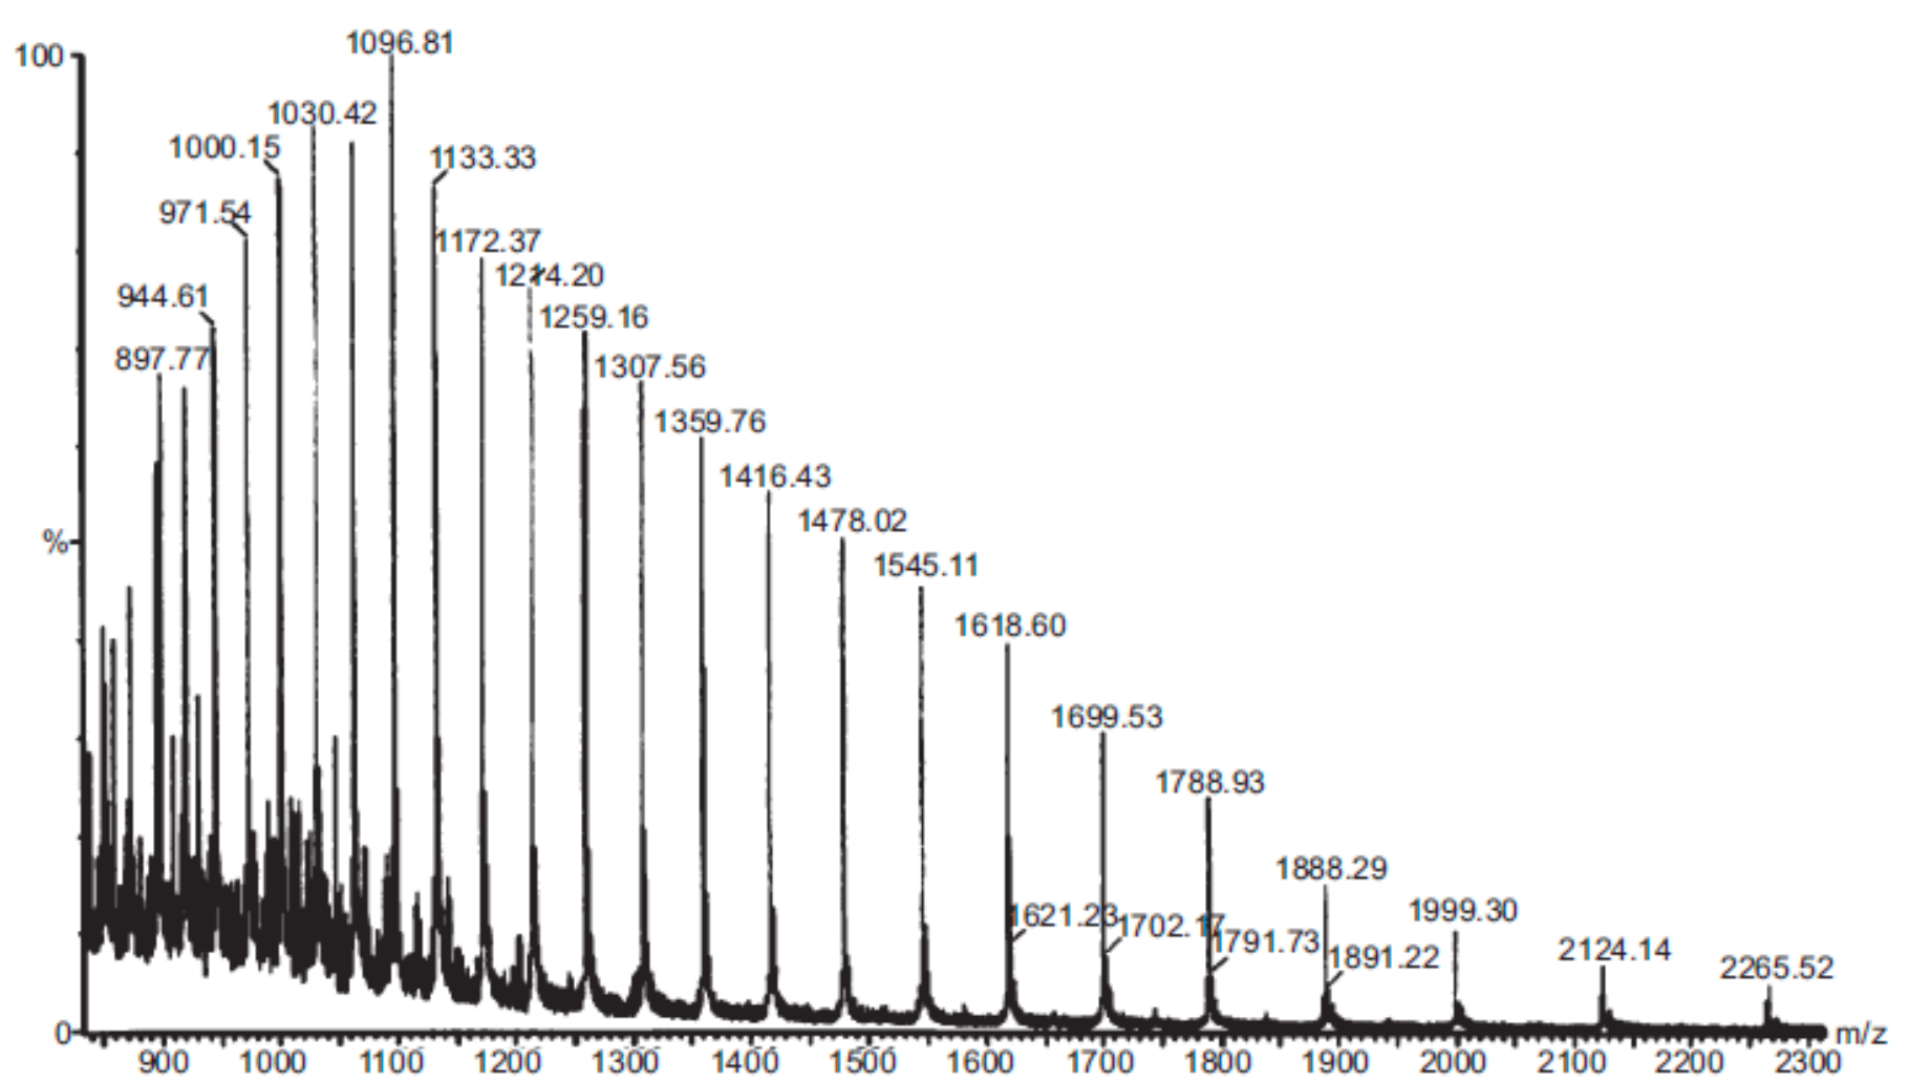
\includegraphics[width=0.92\textwidth]{fig/fig2-mass-spectrum.png}
\end{center}
\noindent\small\textsc{Figure 2} -- Mass spectrum of a protein measured in a spectrometer: the
detected intensity, proportional to the number of ions, as a function of the ratio $m/z$ of the
ions. The mass $m$ is in atomic mass units, which means that it is approximately equal to the
total number of neutrons and protons contained in the protein. [\emph{Principles and
Applications of Clinical Mass Spectrometry}, eds.\ Nader Rifai, Andrea Rita Horvath and Carl
Wittwer, Elsevier, 2018.]\normalsize

\q{13} Recall why the charge of the ion is of the form $q = ze$, where $e$ is the elementary
charge and $z$ a positive integer. Figure~2 shows the distribution of $m/z$ in a sample
analysed by a mass spectrometer. The main peaks correspond to different degrees of ionisation
$z$ of the same protein. Deduce from these data the mass $m$ of the protein. You may begin by
determining the values of $z$ corresponding to the peaks located at $m/z = 1000.15$ and
$m/z = 1999.30$. Estimate the order of magnitude of the number of atoms contained in the
protein.

We now study in detail the technique of ion cyclotron resonance mass spectrometry. It sets in
motion only the ions for which $m/z$ has a precise value, by means of a constant magnetic field
and an electric field oscillating at an angular frequency $\omega$.

\q{14} The ions produced are sent into an analysis cell in which there is a uniform, constant
magnetic field $\vv B = B\,\vv e_z$, where $\vv e_z$ is the unit vector along the $z$ axis and
$B > 0$. Describe a simple experimental device that creates such a magnetic field.

\q{15} Write the equation of motion of the ion under the action of this magnetic field, in
Cartesian coordinates $(x(t), y(t), z(t))$.

\q{16} We introduce the complex coordinate $Z(t) = x(t) + \ii y(t)$. Write the equation of
motion for $Z(t)$, and look for a particular solution of the form
$Z(t) = Z_0\exp(-\ii\omega_0t)$ with $Z_0$ and $\omega_0$ non-zero. Express $\omega_0$ in terms
of $q$, $B$ and $m$. Check your result carefully: it will be used in the rest of the problem.

\subpart{Excitation}

\q{17} By means of an electric field, a time-dependent excitation force perpendicular to the
magnetic field is applied to the ion. Its components are $F_x(t) = F\cos\omega t$ and
$F_y(t) = -F\sin\omega t$. Rewrite the equation of motion for $Z(t)$ taking this forcing into
account.

\q{18} We assume that the ion, of velocity $\vv v$, experiences a friction force
$-(m/\tau)\vv v$ in addition to the magnetic force and the excitation force. This force models
its interaction with the gas contained in the cell. What is the dimension of $\tau$? In what
context have you come across a similar friction force?

\q{19} Write the equation of motion for $Z(t)$ under the combined action of the three forces.
Look for a steady-state (forced) solution of the form $Z(t) = Z_0\exp(-\ii\omega t)$, and
express the amplitude $Z_0$ in terms of $F$, $m$, $\omega$, $\omega_0$ and $\tau$.

\q{20} Show that if the friction force is weak enough, the amplitude $Z_0(\omega)$ exhibits a
resonance at the angular frequency $\omega_0$. Determine the order of magnitude of the width
$\Delta\omega$ of the resonance in terms of $\tau$.

\q{21} The ratio $m/z$ is deduced from a measurement of the resonance angular frequency
$\omega_0$. To distinguish molecules with very close masses, why is it important for $z$ and
the magnetic field $B$ to be as large as possible?

\q{22} In practice, a uniform electric field along the $x$ axis is used,
$E_x(t) = E\cos\omega t$. Show that the excitation force it exerts on the ion can be written as
the sum of two components with angular frequencies $\omega$ and $-\omega$, each of the form of
question~17. Using the previous results, deduce the motion of the ion in the forced regime.
Which of the two components causes the resonance?

\q{23} Describe a simple experimental device that creates such an electric field.

\q{24} We now work exactly at resonance, $\omega = \omega_0$. The friction force is neglected.
Of the two components of the electric field identified in question~22, only the one that
creates the resonance is taken into account. Write the equation of motion for $Z(t)$.

\q{25} Look for a solution of the form $Z(t) = \ii A\,t\exp(-\ii\omega_0t)$, where $A$ is a
constant to be expressed in terms of $E$ and $B$.

\q{26} Sketch the trajectory followed by the ion in the $(x,y)$ plane. You may first write its
equation in polar coordinates in the form $r = f(\theta)$. Describe the respective roles of the
electric and magnetic fields in the motion.

\q{27} We shall see below that the ions are easier to detect at resonance when the amplitude of
their motion is larger. On the other hand, we want to prevent them from leaving the analysis
cell, whose characteristic size $d$ is a few centimetres. Estimate, as a literal order of
magnitude, the optimal value of the time $t_E$ during which the electric field should be
applied, in terms of $d$, $E$ and $B$.

\q{28} We have described a device in which the electric field and the magnetic field are both
uniform. Of these two uniformity conditions, which one seems to you the more important?

\q{29} The ions entering the analysis cell have a thermal motion before being accelerated by
the electric field. Estimate the literal order of magnitude of the corresponding momentum in
terms of $m$ and the temperature $T$.

\q{30} Deduce the order of magnitude of the radius $r$ of the trajectory in the plane
perpendicular to the magnetic field $\vv B$. Excitation by the electric field is effective
only if this initial radius $r$ is much smaller than the characteristic size $d$ of the cell.
Show that this condition holds only if the mass $m$ is much smaller than a critical mass
$m_{\max}$, to be expressed in terms of $q$, $B$, $d$ and $T$.

\subpart{Trapping}

\q{31} Explain briefly why, with the device described above, the ions can escape in the $z$
direction.

\q{32} In addition to the fields already mentioned, electrodes create an electrostatic
potential of the form $V(x,y,z) = \frac\alpha2(-x^2 - y^2 + \beta z^2)$ inside the analysis
cell, with $\alpha > 0$. Write the components of the electric field $\vv E$ corresponding to
this so-called ``trapping'' potential. The cell is assumed to be free of charge. Determine the
value of $\beta$.

We now study the effect of the trapping potential on the motion of the ions. In questions~33
to~36, neither the excitation force nor the friction force is taken into account.

\q{33} Show that the ion oscillates along the $z$ direction about the origin at an angular
frequency $\omega_p$, to be expressed in terms of $q$, $m$ and $\alpha$.

\q{34} Establish how the equation of motion for $Z(t) = x(t) + \ii y(t)$ obtained in
question~16 is modified in the presence of the potential $V(x,y,z)$.

\q{35} Look for particular solutions of the form $Z(t) = Z_0\exp(-\ii\omega t)$ with $Z_0$
non-zero. The trapping field is assumed weak enough for the condition $\omega_p \ll \omega_0$
to hold. Show that there are then two real solutions for $\omega$, denoted $\omega_+$ and
$\omega_-$, with $\omega_+ > \omega_-$, and simplify their expressions in the limit
$\omega_p \ll \omega_0$.

\q{36} Show that the trapping field leads to a small change in the resonance angular frequency.
Show also that a new, much slower oscillatory motion appears in the plane perpendicular to the
magnetic field, and that its frequency is independent of the ratio $m/q$.

\subpart{Detection}
After an electric excitation force has been applied for a time $t_E$, we want to measure the
motion of the ions. To do so, two detection electrodes are placed at $y = -d/2$ and
$y = d/2$. They are identical metal plates of area $S$, at zero electrostatic potential and
connected to each other. We shall show that the motion of an ion in the cell induces a current
between these electrodes. This current oscillates at the angular frequency of the ion's motion
and can be measured.

To this end, we first need to prove a preliminary lemma, with no apparent connection to the
problem under study.

\q{37} Consider a system of $N$ point charges $q_i$ located at positions $\vv r_i$, with
$i = 0,\dots,N-1$. Write the expression of the electrostatic potential $V_i$ created at the
point $\vv r_i$ by the $N-1$ other charges $q_j$, with $j\ne i$.

\q{38} Now consider $N$ charges with different values $q'_i$, but located at the same positions
$\vv r_i$. Denote by $V'_i$ the electrostatic potential created at $\vv r_i$ by the $N-1$ other
charges $q'_j$. Prove the relation $\sum_{i=0}^{N-1}q_iV'_i = \sum_{i=0}^{N-1}q'_iV_i$, known
as the reciprocity theorem.

We accept that this result remains valid if some of the point charges are replaced by
electrodes of arbitrary shape whose positions remain fixed. Then $q_i$ denotes the total charge
carried by the electrode, and $V_i$ its potential. In the case of interest, there are two
electrodes at $y = -d/2$ and $y = d/2$, labelled by the indices $i = 1$ and $i = 2$. The point
charge is labelled by the index $i = 0$; it is at $y = y_0$, with $-d/2 < y_0 < d/2$.

In the configuration of the experiment, the electrodes are at zero potential, so
$V_1 = V_2 = 0$, and the point $y_0$ carries a charge $q$, so $q_0 = q$. We want to determine
the charge difference between the two electrodes, $q_2 - q_1$.

\q{39} To this end, we consider a different charge distribution, in which there is no charge at
$y_0$, so $q'_0 = 0$, and the conductors are held at potentials $V'_1 = -V/2$ and
$V'_2 = V/2$. Determine the potential $V'_0$ at the point $y_0$.

\q{40} By applying the reciprocity theorem, deduce the charge difference $\Delta q = q_2 - q_1$
in terms of $q$, $y_0$ and $d$. Explain briefly how this device makes it possible to determine
the resonance frequency.

\q{41} For what practical reason are the detection electrodes placed perpendicular to the $y$
axis rather than, for example, the $x$ axis?

\q{42} In practice, the excitation electric field does not oscillate at a single angular
frequency but covers a whole range of frequencies. This makes it possible to analyse a range of
values of $m/z$ simultaneously, as in figure~2. Each frequency sets in motion the ions that are
at resonance. After the end of the excitation, the measured variation of $\Delta q(t)$ with
time $t$, which results from the motion of these ions, is also a superposition of a range of
frequencies. The frequencies present can be reconstructed by spectral analysis, by digitising
$\Delta q(t)$ at regular time intervals. Calculate the minimum sampling frequency needed to
obtain the spectrum of figure~2 with a magnetic field $B = 7$~T. Given:
$e/m_u = 10^8~\mathrm{C\cdot kg^{-1}}$, where $m_u$ denotes the atomic mass unit.

\q{43} From the point of view of detection, what is one further advantage of working with
highly charged ions, such as those produced by electrospray, beyond the one already pointed out
in question~21?

\begin{center}$\ast\ast\ast$\\$\ast$\end{center}
\end{document}
